\documentclass[10pt,oneside]{article}

\usepackage[T1]{fontenc}
\usepackage{fontawesome}

\usepackage[paper=a4paper,margin=2cm,bottom=2.5cm]{geometry}
\usepackage[sfdefault,light,condensed]{roboto}
\usepackage[export]{adjustbox}
\usepackage[usenames,dvipsnames,table]{xcolor}

\usepackage{amsmath,amssymb,array,fancyhdr,graphicx,enumitem,lastpage,multicol,tabularx,textcomp,titlesec}
\usepackage{mathtools}

\setlength\extrarowheight{1pt}
\setlength\parindent{0cm}
\renewcommand\headrule{}
\setlength{\footskip}{1.25cm}

\pagestyle{fancy}

\definecolor{BoxHeaderBG}{RGB}{50, 50, 50}
\definecolor{BoxHeaderText}{RGB}{255, 255, 255}

\newcommand{\BoxHeader}[2]{
    \multicolumn{#1}{| >{\bfseries\footnotesize\cellcolor{BoxHeaderBG}\arraybackslash}l |}{
        \textcolor{BoxHeaderText}{#2}
    }
}

\definecolor{ATLHeaderBG}{RGB}{65, 190, 30}
\definecolor{ATLHeaderText}{RGB}{0, 0, 0}

\definecolor{ATLSkillBG}{RGB}{215, 230, 210}
\definecolor{ATLSkillText}{RGB}{0, 0, 0}

\definecolor{DefinitionBoxHeaderBG}{RGB}{30, 30, 110}
\definecolor{DefinitionBoxHeaderText}{RGB}{255, 255, 255}

\definecolor{FormativeHeaderBG}{RGB}{150, 30, 150}
\definecolor{FormativeHeaderText}{RGB}{255, 255, 255}

\definecolor{GlobalContextHeaderBG}{RGB}{255, 255, 150}
\definecolor{GlobalContextHeaderText}{RGB}{0, 0, 0}

\definecolor{KeyConceptHeaderBG}{RGB}{15, 225, 225}
\definecolor{KeyConceptHeaderText}{RGB}{0, 0, 0}

\definecolor{RelatedConceptHeaderBG}{RGB}{15, 170, 170}
\definecolor{RelatedConceptHeaderText}{RGB}{0, 0, 0}

\definecolor{QuestionHeaderBG}{RGB}{240, 240, 240}
\definecolor{QuestionHeaderText}{RGB}{0, 0, 0}

\definecolor{SolutionHeaderBG}{RGB}{225, 150, 110}
\definecolor{SolutionHeaderText}{RGB}{0, 0 , 0}

\definecolor{SummativeHeaderBG}{RGB}{195, 15, 15}
\definecolor{SummativeHeaderText}{RGB}{255, 255, 255}

\newcommand{\ATLHeader}[1]{
    \cellcolor{ATLHeaderBG}\textcolor{ATLHeaderText}{
        \bfseries\footnotesize
        ATL SKILL (#1) \hfill \faGears
    }
}

\newcommand{\ATLSkill}[1]{
    \cellcolor{ATLSkillBG}\textcolor{ATLSkillText}{
        \itshape #1
    }
}

\newcommand{\DefinitionBoxHeader}{
    \cellcolor{DefinitionBoxHeaderBG}\textcolor{DefinitionBoxHeaderText}{
        \bfseries\footnotesize
        DEFINITIONS \hfill \faPencil
    }
}

\newcommand{\FormativeHeader}{
    \cellcolor{FormativeHeaderBG}\textcolor{FormativeHeaderText}{
        \bfseries\footnotesize
        FORMATIVE ASSESSMENT \hfill \faComments
    }
}

\newcommand{\GlobalContextHeader}[1]{
    \cellcolor{GlobalContextHeaderBG}\textcolor{GlobalContextHeaderText}{
        \bfseries\footnotesize
        GLOBAL CONTEXT (#1) \hfill \faGlobe
    }
}

\newcommand{\KeyConceptHeader}[1]{
    \cellcolor{KeyConceptHeaderBG}\textcolor{KeyConceptHeaderText}{
        \bfseries\footnotesize
        KEY CONCEPT (#1) \hfill \faKey
    }
}

\newcommand{\RelatedConceptHeader}[1]{
    \cellcolor{RelatedConceptHeaderBG}\textcolor{RelatedConceptHeaderText}{
        \bfseries\footnotesize
        RELATED CONCEPT (#1) \hfill \faLink
    }
}

\newcommand{\SolutionHeader}[1]{
    \cellcolor{SolutionHeaderBG}\textcolor{SolutionHeaderText}{
        \bfseries\footnotesize 
        #1 \hfill \faPaste
    }
}

\newcommand{\SummativeHeader}{
    \cellcolor{SummativeHeaderBG}\textcolor{SummativeHeaderText}{
        \bfseries\footnotesize
        SUMMATIVE ASSESSMENT \hfill \faCheck
    }
}

\newcounter{QuestionCounter}

\newcommand{\QuestionBox}[1]{
    \stepcounter{QuestionCounter}
    \cellcolor{QuestionHeaderBG}\textcolor{QuestionHeaderText}{
        {\bfseries\scriptsize Q\theQuestionCounter} #1
    }
}

\newcommand{\boxwidth}{\linewidth}

\lhead{\scriptsize\texttt{U\UnitNumber: \UnitTitle \\ L\LessonNumber: \LessonTitle}}
\rhead{\scriptsize\ttfamily [DESIGN/\CourseName/U\UnitNumber/L\LessonNumber]\\\ }

\lfoot{
\includegraphics[height=2cm,valign=c]{Files/logo}}
\cfoot{\footnotesize DESIGN/\CourseName/U\UnitNumber/L\LessonNumber\ | \LessonTitle \\ Woodstock School | Mussoorie, Uttarakhand, India}
\rfoot{
\includegraphics[height=2cm,valign=c]{Files/ib-world-school-logo-1-colour}}

\titleformat{\section}{\normalfont\Large\bfseries}{}{0em}{}[{\titlerule[0.5pt]}]
\titleformat{\subsection}{\normalfont\large\bfseries}{}{0em}{}


\usepackage{circuitikz,subcaption}

\def\CourseName{MYP3}

\def\LessonNumber{02}
\def\LessonTitle{Measuring Electricity}

\def\UnitNumber{01}
\def\UnitTitle{Circuits \& Electronics}

\begin{document}
    % Core Components (Remove when no longer required!)
    \thispagestyle{empty}
    \begin{tabularx}{\boxwidth}{| X | }
        \hline
        \ATLHeader{} \\\hline
        \ATLSkill{} \\\hline
        \QuestionBox{} \\\hline
    \end{tabularx}

    \begin{tabularx}{\boxwidth}{| X |}
        \hline
        \DefinitionBoxHeader \\\hline
    \end{tabularx}

    \begin{tabularx}{\boxwidth}{| X |}
        \hline
        \GlobalContextHeader{}\\\hline
    \end{tabularx}

    \begin{tabularx}{\boxwidth}{| X |}
        \hline
        \KeyConceptHeader{} \\\hline
    \end{tabularx}

    \begin{tabularx}{\boxwidth}{| X |}
        \hline
        \RelatedConceptHeader{} \\\hline
    \end{tabularx}

    \begin{tabularx}{\boxwidth}{| X |}
        \hline
        \SolutionHeader{SOLUTION} \\\hline
    \end{tabularx}

    \begin{tabularx}{\boxwidth}{| X | }
        \hline
        \FormativeHeader \\\hline
        \QuestionBox{} \\\hline
    \end{tabularx}

    \begin{tabularx}{\boxwidth}{| X |}
        \hline
        \SummativeHeader \\\hline
        \QuestionBox{}\\\hline
    \end{tabularx}

    \newpage

    \begin{center}
        \huge\bfseries
        \LessonTitle
    \end{center}

    \section{Before You Begin}

    \begin{tabularx}{\boxwidth}{| X |}
        \hline
        \KeyConceptHeader{Development} \\\hline
    \end{tabularx}

    \begin{tabularx}{\boxwidth}{| X |}
        \hline
        \RelatedConceptHeader{Invention} \\\hline
        \QuestionBox{We are examining the invention of electrical circuits as a \emph{turning point} in history. What other inventions do you think resulted in an historical turning point?} \\\hline
        \ \\[3cm]\hline
    \end{tabularx}
    \pagebreak

    \section{Technical Background}

    \subsection{Voltage}
    Voltage, measured in \emph{volts} (\textbf{V}), is a \emph{potential} difference between a positively and negatively charged part of a circuit. A common example illustrating the concept of voltage that of a water tank or tower.

    \begin{figure}[h]
        \centering
        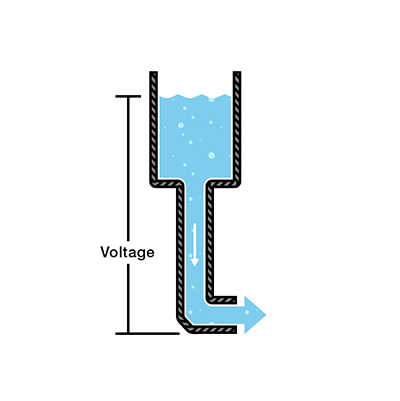
\includegraphics[height=6cm]{Extras/voltage}
        \caption*{\scriptsize Image courtesy sparkfun.com.}
    \end{figure}
    In this illustration, voltage can be seen as equivalent to the \emph{water pressure} coming out of the hose at the bottom of the system. Factors such as the height and size of the tank can have an impact on how much pressure is available. This is the \emph{potential energy} concept. While batteries and other sources of electricity provide power in different ways, the analogy is still useful for understanding what voltage contributes to an electrical circuit.

    \subsubsection*{Voltage Drop / Forward Voltage} 
    \emph{Voltage Drop} or \emph{Forward Voltage} is the amoung of voltage ``consumed'' by a load or other component in an electrical circuit.

    \medskip
    \begin{tabularx}{\boxwidth}{| X |}
        \hline
        \SolutionHeader{Kirchhoff's Voltage Law} \\\hline
        \emph{Kirchhoff's Voltage Law} (or \emph{Kirchhoff's Second Law}) essentially states that sum of all voltage drops in a clossed electrical circuit, such as the simple circuits we built in the previous lesson, will be equal to the voltage of the source.\\\hline
    \end{tabularx}

    \subsection{Current}
    Current, measured in \emph{amperes} (\textbf{A}), is the \emph{flow} of electricity within a circuit. You can think of current as the \emph{speed} at which electricity flows.    

    \medskip
    \begin{tabularx}{\boxwidth}{| X | }
        \hline
        \ATLHeader{Communication Skills} \\\hline
        \ATLSkill{...make inferences and draw conclusions...} \\\hline
        \QuestionBox{Considering the water tank example given above for voltage, what changes to the system would have an impact on the flow of water out of it?} \\\hline
        \ \\[4cm]\hline
    \end{tabularx}

    \subsection{Resistance}
    % Ohm's Law

    \subsection{The Resistor}

    \begin{tabularx}{\boxwidth}{| >{\bfseries}p{0.15\boxwidth} | X | >{\centering\arraybackslash}p{0.15\boxwidth} | >{\centering\arraybackslash}p{0.15\boxwidth}| }
        \hline
        \BoxHeader{1}{Name} & \BoxHeader{1}{Description} & \BoxHeader{1}{Symbol} & \BoxHeader{1}{Example} \\\hline
        Resistor & 
        A \emph{resistor} is an electronic component designed to reduce the current flow in a circuit.

        \medskip
        The \emph{resistance} offered by each resistor is measured in Ohms ($\Omega$).
        & 
        \raisebox{-0.5cm}{
            {\tikz \draw (0, 0) to [R] (2, 0);} 
        }

        \bigskip
        {\tikz \draw (0, 0) to [european resistor] (2, 0);}
        & 
        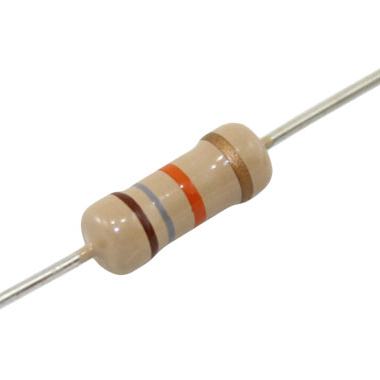
\includegraphics[width=0.9\boxwidth,valign=t]{Extras/resistor}
        \\\hline
    \end{tabularx}

    \medskip
    The type of resistor we will be using are labeled using coloured bands to denote their resistance. You have a copy of the following image in your electronics kits:
    
    \begin{figure}[h]
        \centering
        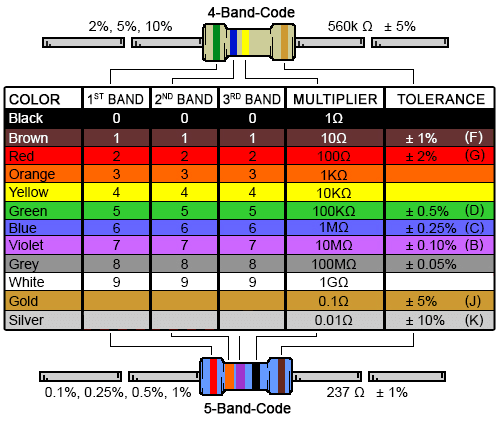
\includegraphics[height=8cm]{Extras/resistor_chart}
        \caption*{\scriptsize Image courtesy digikey.com.}
    \end{figure}

    \begin{tabularx}{\boxwidth}{| X |}
        \hline
        \ATLHeader{Communication Skills} \\\hline
        \ATLSkill{...use and interpret a range of discipline-specific terms and symbols...} \\\hline
        \QuestionBox{In the next section, you'll need one of each of the following resistance value resistors: $220 \Omega$, $1 \text{k}\Omega$, $10 \text{k}\Omega$. These are available in your electronics kit. Determine whether your resistors are $4-$ or $5-$band and identify the correct colour bands for each required value. You can safely ignore the ``tolerance'' band for now.} \\\hline

        \textbf{220 $\mathbf{\Omega}$ \hfill 1 k$\mathbf{\Omega}$ \hfill 10 k$\mathbf{\Omega}$ \hspace{4cm} \,} \\[4cm]\hline
    \end{tabularx}

    \pagebreak

    \section{Developing Technical Skills}
    
    \pagebreak
    
    \section{Reflections}
\end{document}